\subsection{Compiler Overview}\label{subsec:overview}

\begin{figure}
\centering
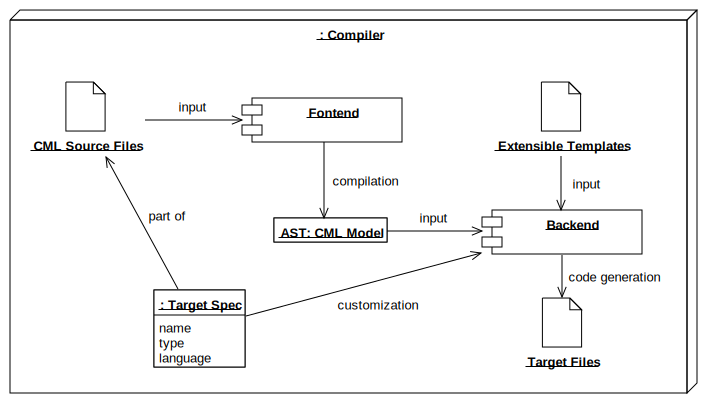
\includegraphics[width=0.8\textwidth]{compiler/figure-overview}
\caption{An architectural overview of the CML compiler.}
\label{fig:overview}
\end{figure}

An overview diagram of the architecture is shown in figure \ref{fig:overview}.
The two main components of the compiler,
and the artifacts they work with,
are presented below:

\begin{itemize}

\item \emph{Frontend:} receives as input the \emph{CML source files}.
It parses the files into an internal representation of the \emph{CML model}.
Syntactical and semantic validations are then executed.
Any errors are presented to the developer, interrupting the progress to the next phase.
If the \emph{source files} are parsed and validated successfully,
the \emph{CML model} serves then as the input to the \emph{backend} component.

\item \emph{Backend:} receives the \emph{CML model} as input.
Based on the \emph{constructor} defined by a \emph{task},
the \emph{backend} chooses which \emph{extensible templates} to use for code generation.
The \emph{target files} are then generated to be consumed by other tools.
The \emph{task} and associated \emph{constructor} play a key role
in determining the kind of \emph{target} to be generated.

\end{itemize}
